\chapter{HERO Architecture Simulation}
\label{chap:results}

To assess the performance of the HERO architecture a cycle accurate simulation
environment was implemented using SystemC and python. The environment was used
to a single configurations of the HERO architecture on real networks implemented
in pytorch from the TIMM library. The simulator also enables a study of the HERO
architecture by allowing different configurations of HERO to be passed in during
simulation. This study is left as part of future work. The simulator is composed
of two parts. 1) A python based frontend that can analyze the performance
results of any pytorch network on a configuration of HERO. 2) A SystemC based
backend for cycle accurate simulations of HERO running convolution/linear layers. In
this chapter we will first discuss the simulation environment and it's
components in \autoref{chap:hero:sim_platform}. The results from simulating all
695 networks from TIMM using a small HERO instance are given
\autoref{chap:hero:results}.

\section{Simulation Environment}
\label{chap:hero:sim_platform}

\subsection{Python Frontend}
\label{chap:hero:sim_platform:frontend}

The python frontend depicted in \autoref{fig:frontend}, expects a list of pytorch models and a dictionary defining the
configuration of a HERO instance as inputs. The configuration specifies the unroll factors
for F, C, the list of kernels sizes supported in direct mode, and the on-chip
storage dedicated for input and output feature map reuse, as well as the maximum
line size in any IFmap tensor.  The output of the
frontend is a pandas dataframe containing the results from the backend
simulation of the network(s) on the specified hero instance.  
After the frontend
receives the list of pytorch models, CIGAR extracts the dimensions of all
supported layers (Conv2D and Linear). After which two layer transformation
operations are performed. The first converts convolution layers that are
unsupported directly into equivalent (1, 1) convolutions as described in
\autoref{chap:dda:dataflow_dse:indirect_mode}. Additionally, linear layers are
reinterpreted as (1, 1) convolutions based on the proof derived from
\autoref{chap:dda:dataflow_dse:indirect_mode:conv_gemm_equiv:proof}. 
The HERO arch. config being
evaluated is used to determine what layers are supported directly
After all layers have been converted to equivalent layers
that are supported by HERO, a layer decomposition step is performed to
decompose layers that have featuremaps that are two large to fit in the
HERO's on-chip memory. 
After all layer transformations are
performed, the layers are converted to test cases and a testcase deduplication
operation is used to limit the number of simulation runs required to simulate the network(s)
on HERO. 
After the testcase queue is generated it gets passed off to several
worker threads that manage independent backend instances that simulate the different
layers of the input network(s) concurrently. Note that since we're only
concerned with the architecture metrics produced by the simulation the layers being
simulated don't use real weights and featuremaps from a forward inference pass
of the original network. Instead equivalent layer weights and featuremaps are
instantiated in the backend to avoid unnecessary transfer of data between the
front and backend.      


\begin{figure}[ht]
    \centering
    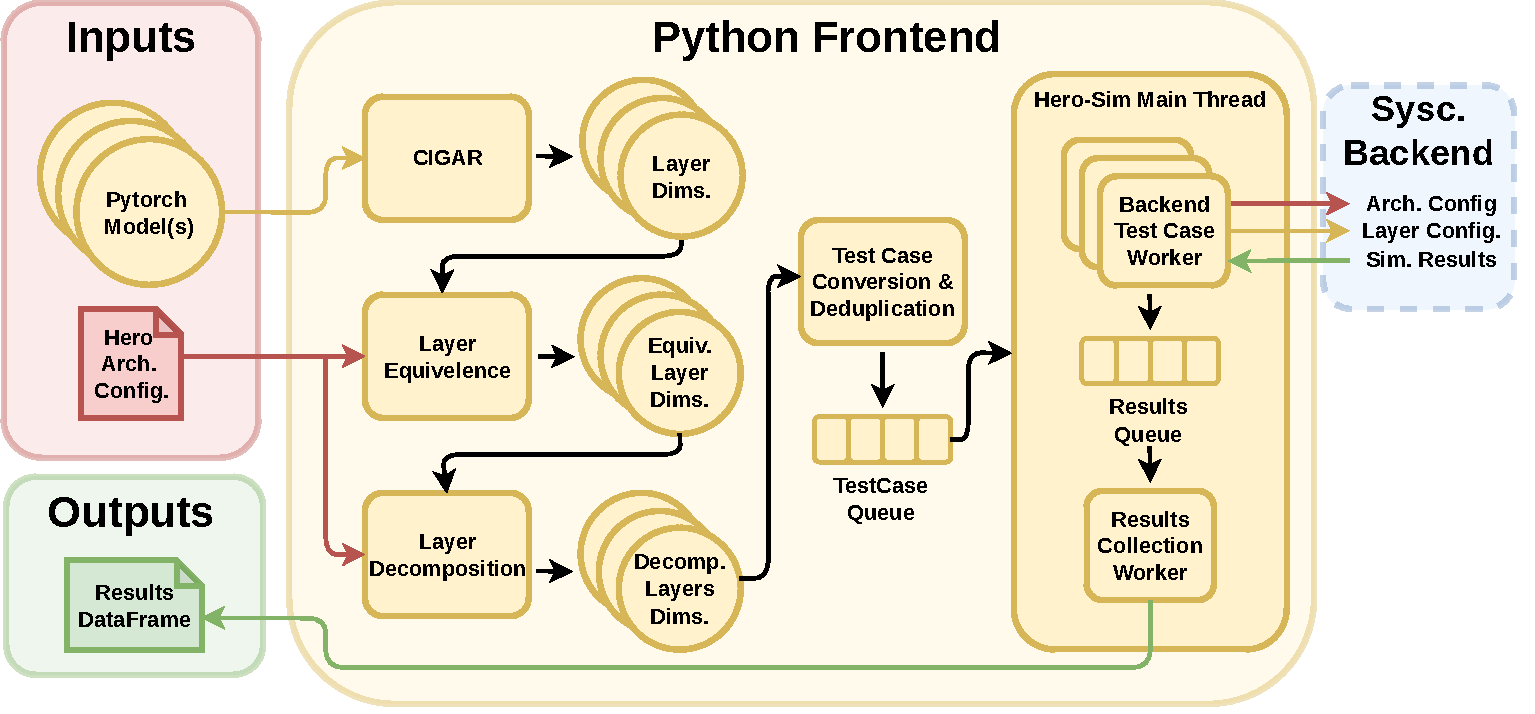
\includegraphics[scale=0.58]{fig/hero-sim-frontend.pdf}
    \caption{Illustration of the simulation environment's python frontend}
    \label{fig:frontend}
\end{figure}


\subsection{SystemC backend}
\label{chap:hero:sim_platform:backend}

The SystemC backend depicted in \autoref{fig:backend}, expects all inputs to be passed in as command line
arguments. The main inputs are 1) architecture configuration and 2) layer
configuration needed for simulation by the frontend. Sim results are generated
and sent back to the frontend using protobufs. The backend first instantiates a
HERO instance using the architecture configuration passed as input. Then it
generates an equivalent layer based on the input layer configuration. Finally
using both layer and architecture configuration it generates the SAM descriptors
required to perform all data movement operations on-chip. A dram load is then
simulated in zero time to transfer the layer data and descriptors to the on-chip
memories of the newly constructed HERO instance. Once the initialized HERO
instance is ready, the cycle accurate simulation starts and continues until all
SAMs reach a suspend descriptor. Then a dram load operation is again performed
in zero time to transfer the results from the HERO instance for validation.
After the simulated dram load, a protobuf is constructed, then populated with
the result of output validation and simulation results (assuming validation
success) and sent back to the frontend for further analysis and aggregation. 

The backend simulates interactions between the architecture and DRAM
functionally, in zero-time to avoid the complexity of DRAM and SAM interactions.
The interaction between SAMs and DRAM are left as part of future work. 

\begin{figure}[ht]
    \centering
    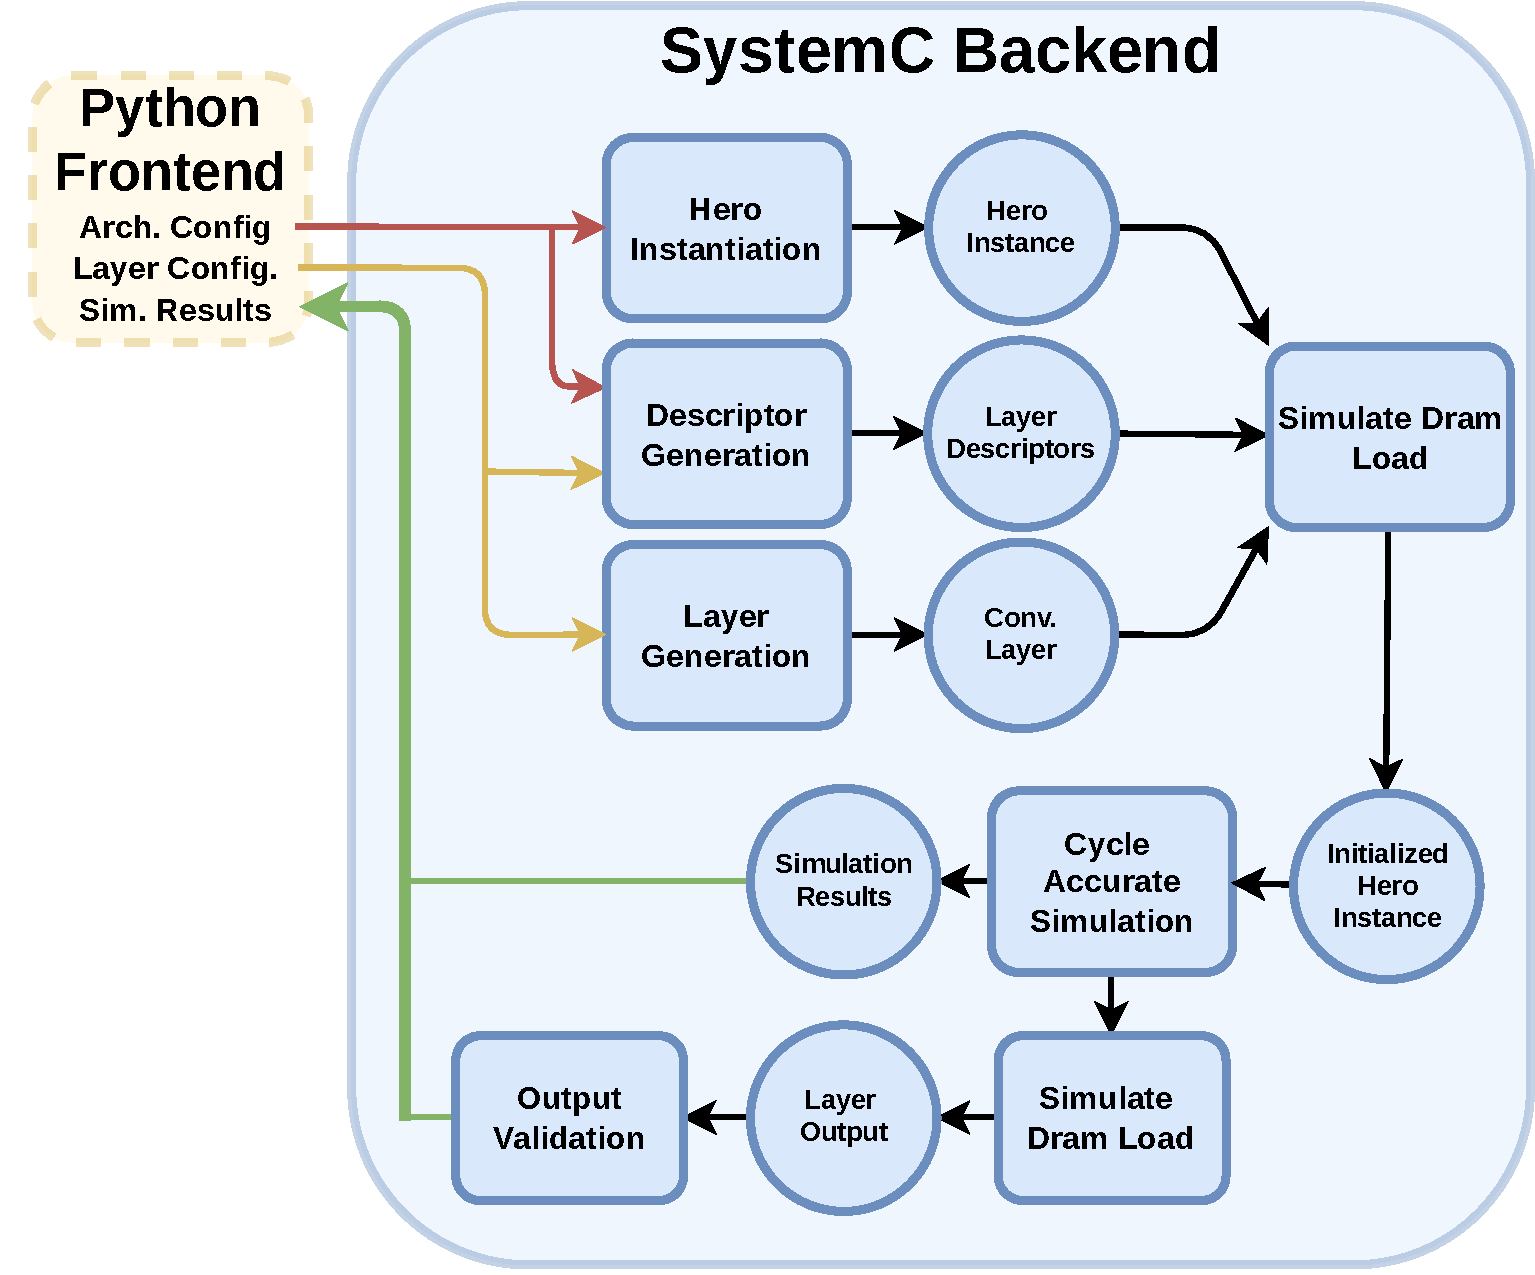
\includegraphics[scale=0.5]{fig/hero-sim-backend.pdf}
    \caption{Illustration of the simulation environment's SystemC backend}
    \label{fig:backend}
\end{figure}

\section{Experimental Results}
\label{chap:hero:results}

The configuration for the simulated architecture is given in
\autoref{tab:hero_config} based on the dimensions discovered in
\autoref{chap:dataflow_dse:exploring:results} and the sizing conclusions from
\autoref{chap:dataflow_dse:memory_hierarchy_sizing}. Note that other larger HERO
variants could have been chosen for this work, however, to minimize simulation
time and to explore a variant of HERO fit for more constrained embedded
environments the configuration in \autoref{tab:hero_config} were chosen.   
Note that sizes for on-chip
storage are given in the aggregate. The number of banks for IFmap L3 and OFmap
storage scales with the chosen $F_{unroll}$ and $C_{unroll}$ factors. As a
result, the size of individual IFmap L3 and OFmap bank is proportional with the
overall size of IFmap L3 and OFmap on-chip storage but inversely proportional
with the chosen unroll factors. The CPU baseline used in this work is an AMD
5950X processor. To minimize simulation time the frontend takes advantage of the
similarity between layer configurations across networks in the timm library.
The total number of both convolution and linear layers post layer configuration
deduplication is reduced from 182773 to 6048. This enables a simulation time of
less than 1.5 hours for all 695 Networks.

\begin{figure}[ht]
    \centering
    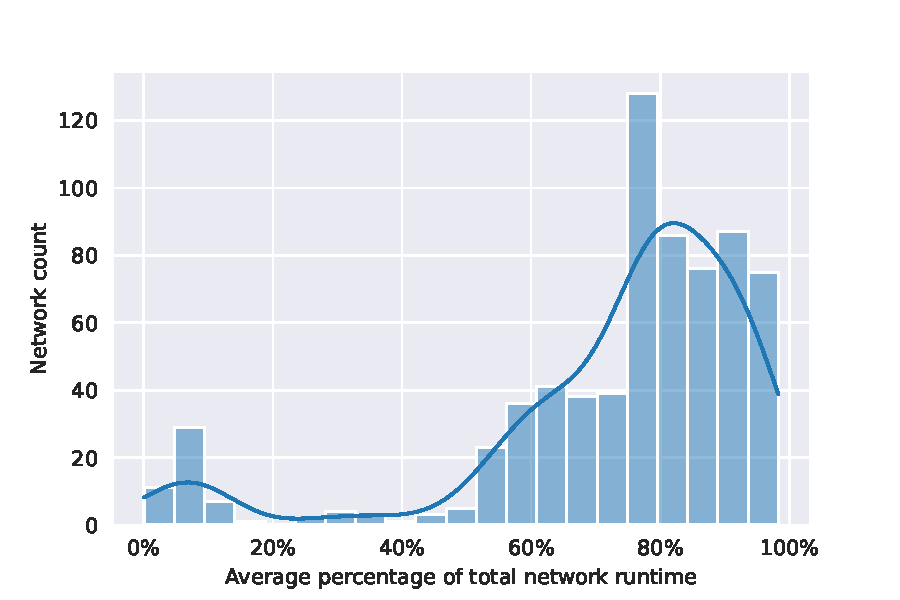
\includegraphics[scale=0.58]{Plots/overview/percent.pdf}
    \caption{Percent of computation represented by layers studied in the TIMM library}
    \label{fig:percent_of_compute}
\end{figure}

The layers simulated (convolution and linear) represent a substantial portion of
total network computation as show in \autoref{fig:percent_of_compute}. 
To determine percentage of compute Pytorch can be used to estimate the
total number of MAC operations used by natively supported layers. Unfortunately
many networks use custom layers constructed with pytorch primitives. For
each of these layers an analytical expression would need to be created to calculate
the number of operations in these layers. For simplicity the runtime
of these layers on a CPU were used to estimate computational demand. In
\autoref{fig:percent_of_compute}, the horizontal access defines the average
percentage of total network runtime taken up by supported layers. The vertical
axis defines the number of networks where convolution and linear layers take up
x\% of the computation where x is defined on the horizontal axis. From
\autoref{fig:percent_of_compute} it can be seen that the convolution and linear
layers represent the majority of network runtime in the TIMM library. 

\begin{table}[]
    \center
    \begin{tabular}{|l|l|}
    \toprule
    Config. Param. & On-Chip Storage in Bytes    \\ 
    \midrule
    Weight Storage            & 16 B / PE (8 bit precision)  \\ \hline
    IFmap L3 Storage          & ~1 MB (8 bit precision)   \\ \hline
    IFmap L2 Storage          & 512 B (8 bit precision)   \\ \hline
    OFmap Storage             & 2 MB (16 bit precision)   \\ \hline
    $C_{unroll}$              & 18   \\ \hline
    $f_{unroll}$              & 32   \\ \hline
    Directly Supported Kernels             & {(1, 1), (3, 3)}   \\ \hline
    Assumed CLK Speed             & 1 Ghz   \\ \hline
\end{tabular}
\caption{HERO configuration used for analysis}
\label{tab:hero_config}
\end{table}

\subsection{Utilization}
\label{chap:hero:results:utilization}

Utilization can be used as a surrogate for how well layers map to the selected
HERO architecture based on the dataflow optimizations discussed in
\autoref{chap:arch_dimensioning}. From figure
\autoref{fig:network_layer_level_utilization} we can see that some networks benefit substantially from the architecture while
others don't. Network level distribution of average layer utilization is generally flat with
about a third of networks not benefiting from the architecture due to low
utilization. Low utilization is defined as average PE utilization throughout a
layer's computation that's less than 50\%.  


\begin{figure}
    \centering
    \subfigure[]{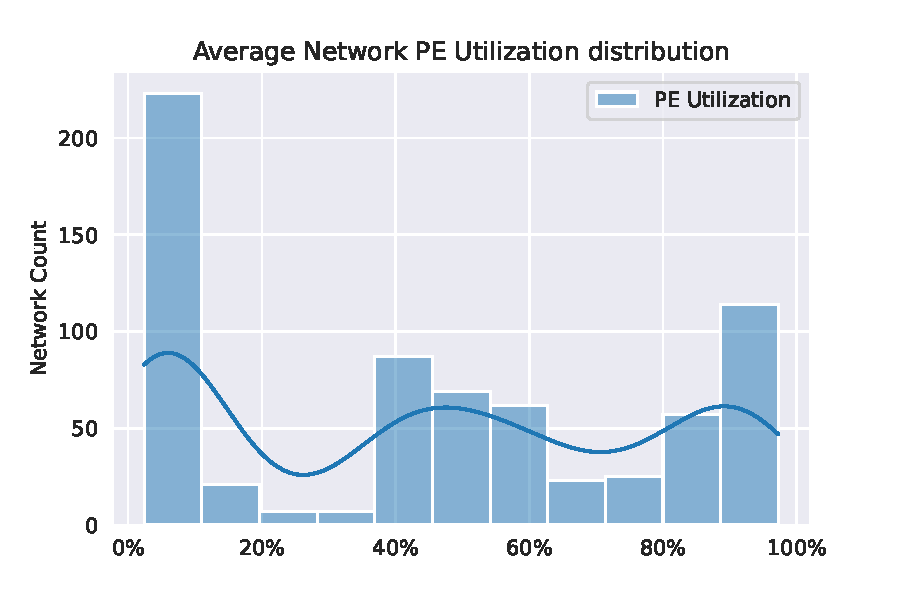
\includegraphics[width=0.48\textwidth]{Plots/utilization/network.pdf}}
    \hspace{0.1cm} 
    \subfigure[]{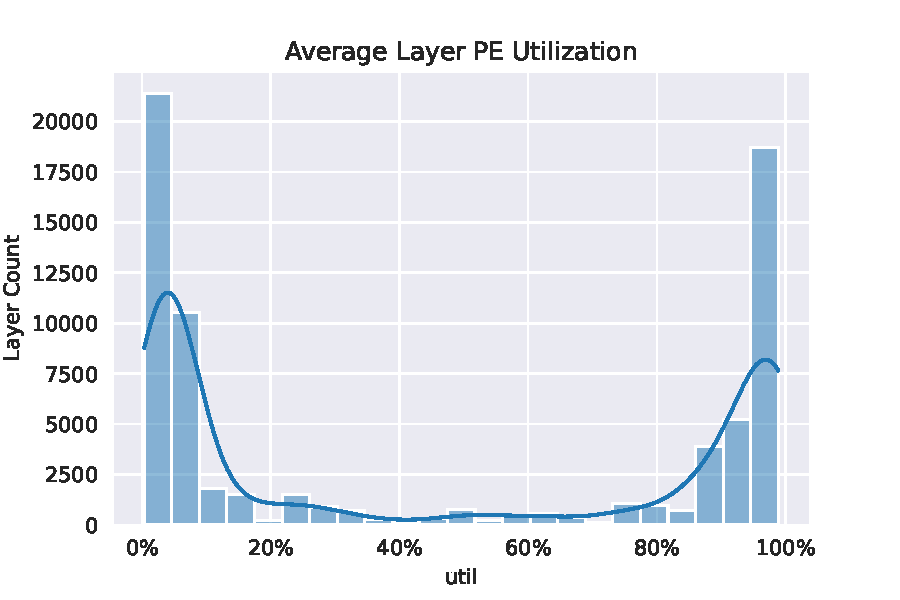
\includegraphics[width=0.48\textwidth]{Plots/utilization/layers.pdf}}
    \caption{Average layer utilization distributions by a) Network, b)Layer}
    \label{fig:network_layer_level_utilization}
\end{figure}

At the layer level we can see a more pronounced disparity in how much the
architecture benefits some layers over others. The next series of figures will
explore the cause of this disparity in utilization. If the cause of low
utilization in most layers is layer size as defined by number of operations then
utilization would generally scale with number of operations. Figure
\autoref{fig:utilization_macs_scaling} shows that the expected trend of
utilization scaling with MACS generally holds. However for a portion of the
layers on the bottom right utilization is low while MACs ops are high. This low
utilization would be especially concerning if combined with a speedup factor
$<1X$ over CPU baseline for that layer. One possible cause of low utilization,
combined with high MAC OPs and low speedup could be a high layer memory
footprint. To examine the effect of layer memory footprint as a cause for low
utilization, a scatter plot of layer feature map size vs utilization is
presented in \autoref{fig:scatter_plot_util_vs_fmap} for layers where speedup
was <1 compared to the CPU baseline. 


\begin{figure}[ht]
    \centering
    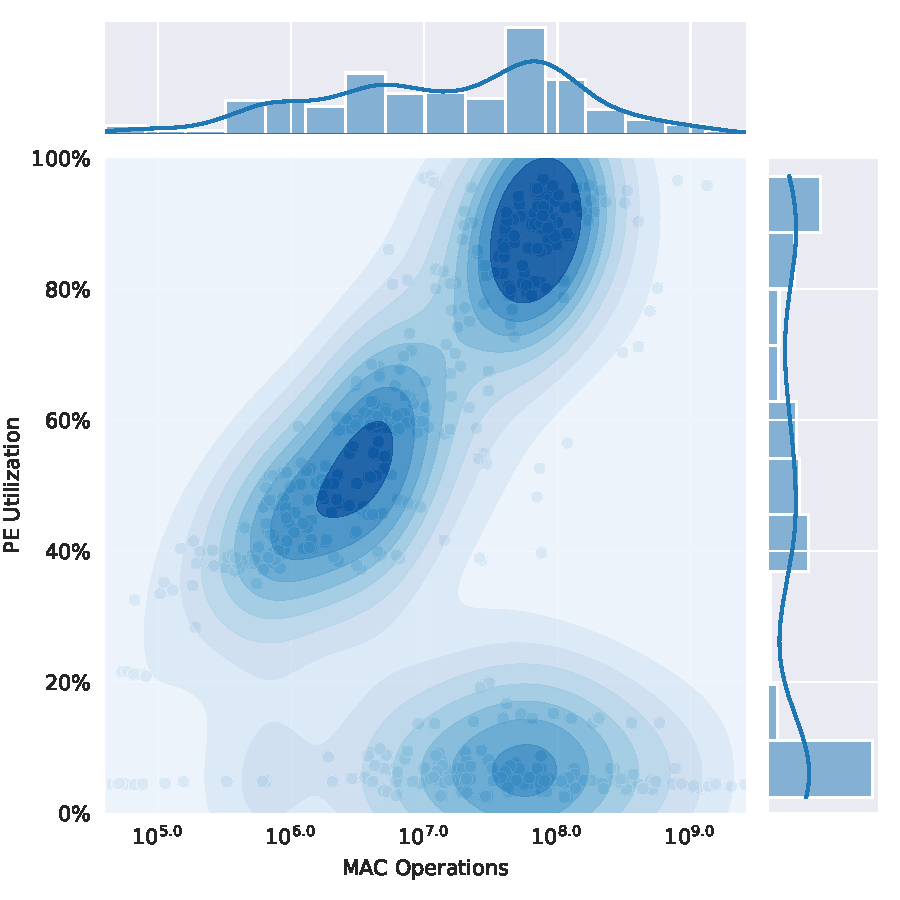
\includegraphics[scale=0.58]{Plots/utilization/util_vs_macs.pdf}
    \caption{Shaded contour plot of average layer utilization vs number of MACs}
    \label{fig:utilization_macs_scaling}
\end{figure}

From \autoref{fig:scatter_plot_util_vs_fmap} it's clear that layer memory
footprint does not correlate with low utilization. What does correlate low
utilization is layer type. The majority of low utilization layers are depthwise
convolution layers as in figure \autoref{fig:cause_of_low_util}.a. Depthwise
layers were not considered during dataflow DSE in \autoref{chap:dda}. Since they
weren't an optimization target the frontend decomposes depthwise layers into
individual groups of convolutions and since depthwise layers are convolution
layers where each IFmap channel is convolved with a kernel independently of the
others, all PEs dedicated to concurrent channel processing are underutilized.
From \autoref{fig:cause_of_low_util}.a there a few non grouped convolution
layers with low low utilization and low speedup. These layers when examined more
closely in \autoref{fig:cause_of_low_util}.b and they appear to have lower
available channel/ filter concurrency as defined by the number of channels/
filters in a layer relative to the available effective channel/ filter
concurrency of the architecture. In both cases of depthwise/grouped convolutions
and low channel/filter count non-grouped convolutions, low utilization and low
speedup can be remedied by exploiting other forms of concurrency in the
architecture other that Filter/Channel/Kernel concurrency chosen by HERO. 

\begin{figure}
    \centering
    \subfigure[]{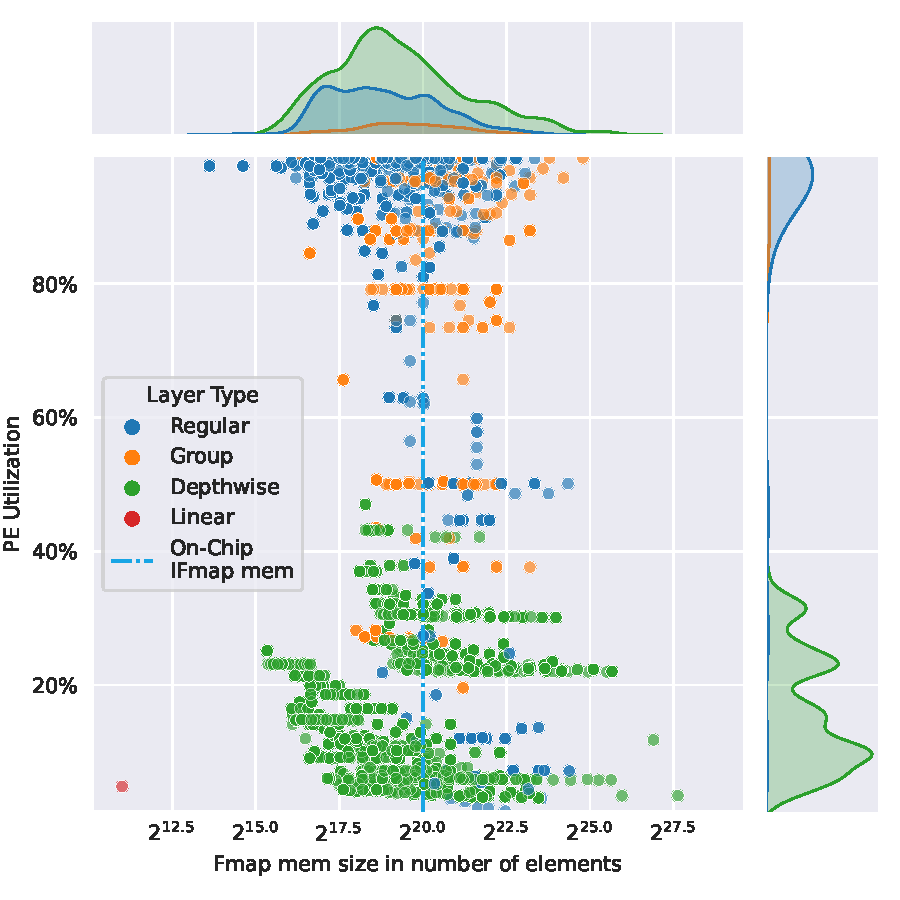
\includegraphics[width=0.48\textwidth]{Plots/utilization/util_vs_ifmap.pdf}}
    \hspace{0.1cm} 
    \subfigure[]{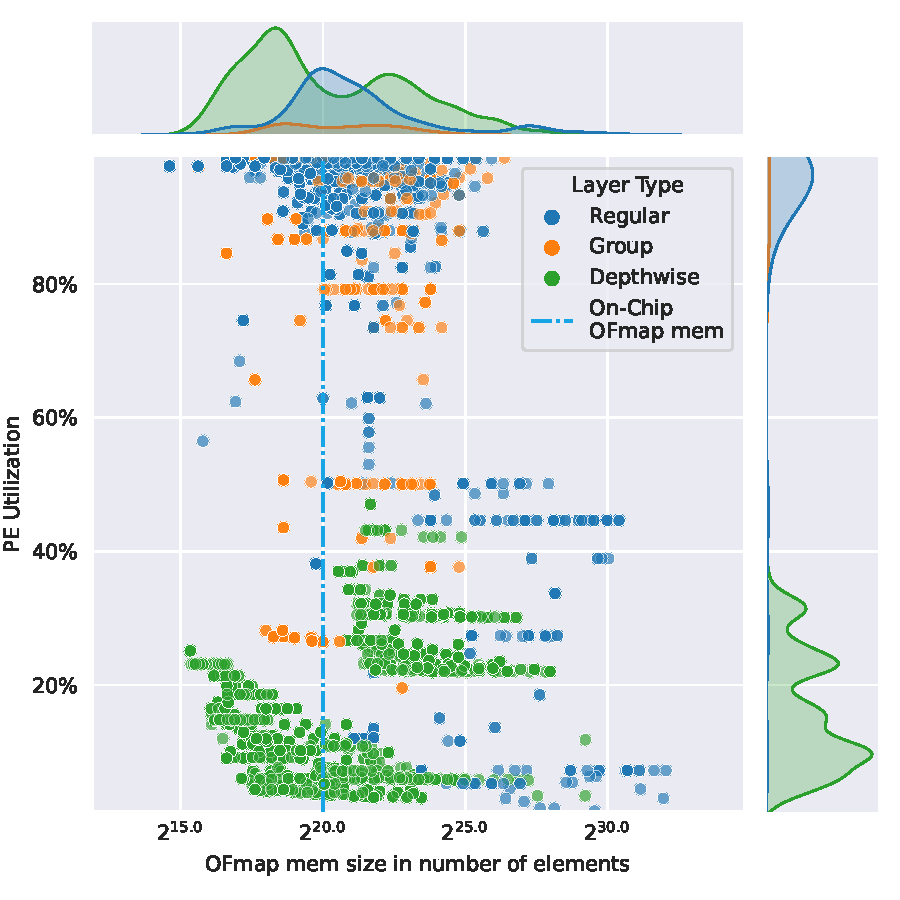
\includegraphics[width=0.48\textwidth]{Plots/utilization/util_vs_ofmap.pdf}}
    \caption{Scatter plot of utilization vs layer a) IFmap size and b) OFmap size. The dotted blue line represents the on-chip memory allocated for both types of feature maps.}
    \label{fig:scatter_plot_util_vs_fmap}
\end{figure}

\begin{figure}
    \centering
    \subfigure[]{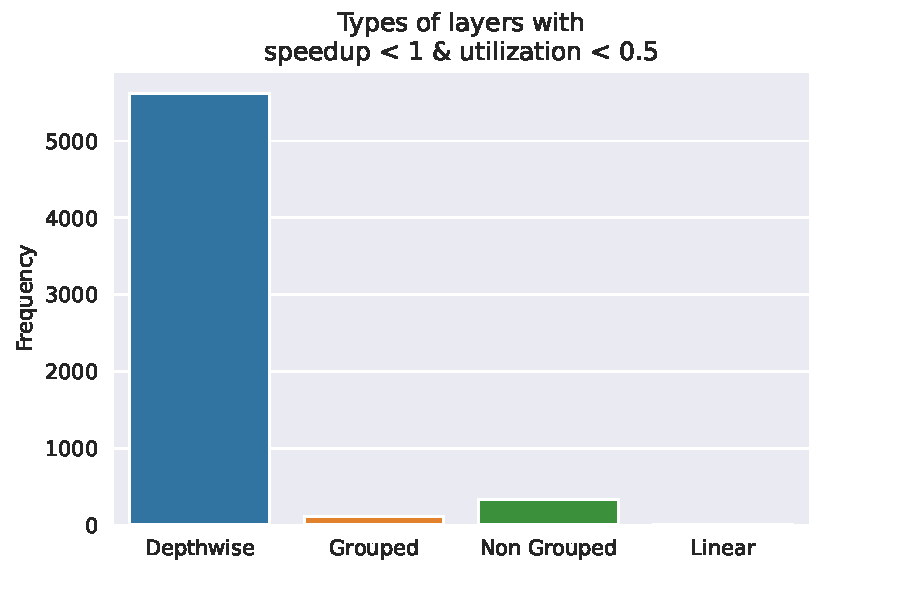
\includegraphics[width=0.48\textwidth]{Plots/utilization/type_of_low_util.pdf}}
    \hspace{0.1cm} 
    \subfigure[]{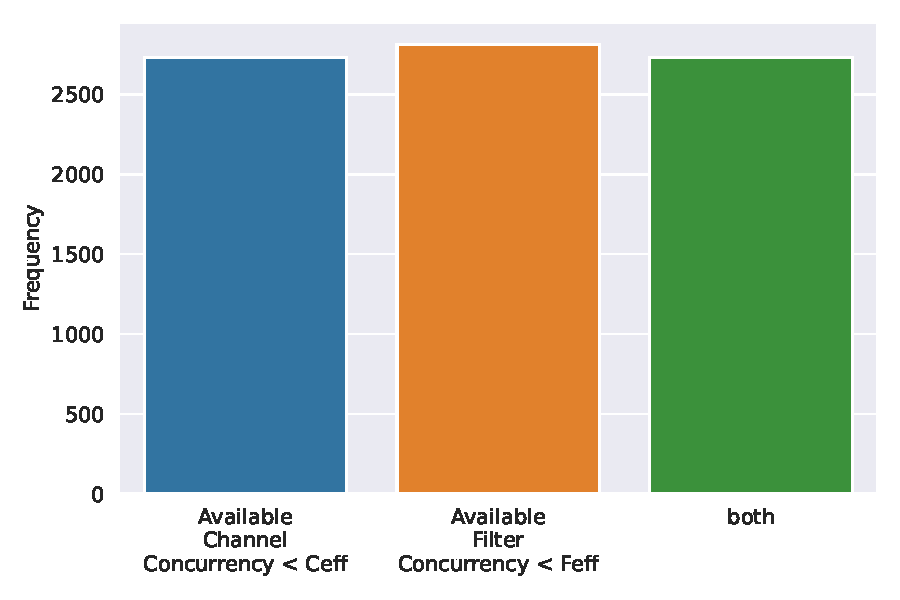
\includegraphics[width=0.48\textwidth]{Plots/utilization/low_util_big_fmap.pdf}}
    \caption{Illustration of the causes of low utilization due to A) Layer type and B) Layer dimensions}
    \label{fig:cause_of_low_util}
\end{figure}

Paradoxically, \autoref{fig:scatter_plot_util_vs_fmap} shows a cluster with
layers with both high utilization and low speedup relative to the CPU baseline.
When examining the Channel and Filter counts for these layers in
\autoref{fig:mac_ratios}.a it can be seen that they are generally multiple orders
of magnitude greater than the available effective channel/ filter concurrency.
In effect these layers suffer from the opposite problem of the previous layers.
The resources allocation defined in \autoref{tab:hero_config} is too low to
satisfy the available filter and channel concurrency in these high utilization
but low speedup layer. 
The impact of lowering and lifting on increasing the number of MAC operations of
a layer cannot be understated. When comparing the CPU baseline vs HERO, the CPU
baseline has the inherent advantage of a larger and more complex memory
hierarchy that enables more complicated access patterns to occur. This advantage
allows CPUs to support arbitrary layers without relying on lowering/ lifting
data transformations which can dramatically increase the effective number of MAC
operations in a layer as seen in \autoref{fig:mac_ratios}.b where the median MAC
factor increase as a result of the balanced lowering/ lifting scheme chosen by
HERO is ~3.8X over the original number of MACs present in the layer. In short
HERO has to perform more operations for the same layers relative to CPU. To
remedy this issue, more layers need to be supported directly by HERO.  

\begin{figure}
    \centering
    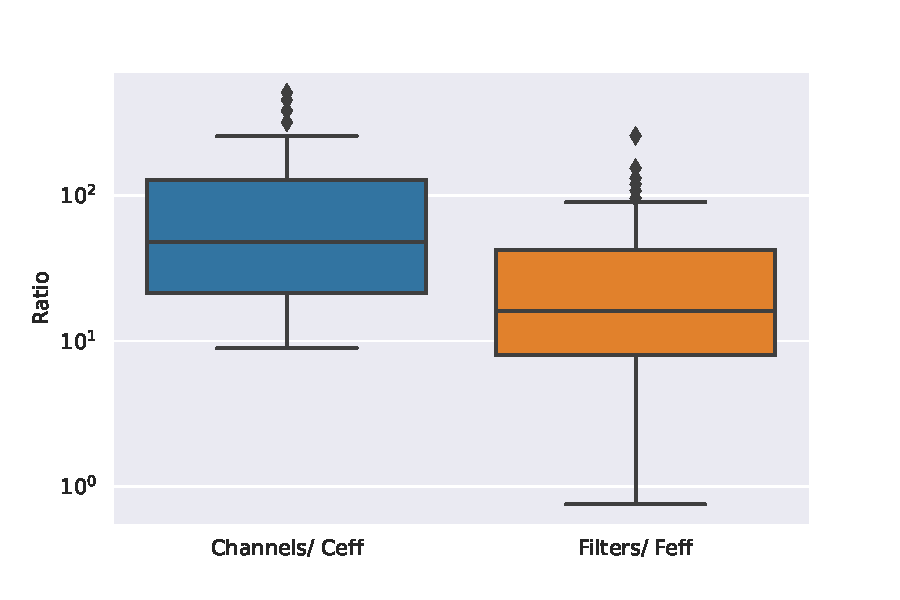
\includegraphics[scale=0.48]{Plots/utilization/ratios.pdf}
    \hspace{0.1cm} 
    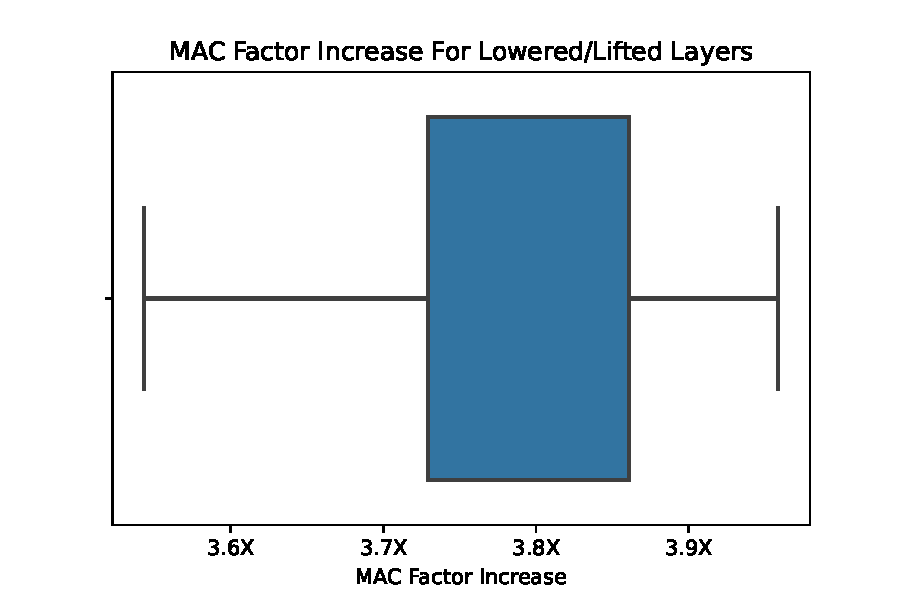
\includegraphics[scale=0.48]{Plots/utilization/macs.pdf}
    \caption{A) Barplot of the ratios between layer channel/ filters vs effective available channel/ filter concurrency for layers with speedup $<$ 1 and utilization $>$ 95\% b) Barplot of the MAC factor increase due to lowering/lifting for layers with speedup $<$ 1 and utilization $>$ 95\%}
    \label{fig:mac_ratios}
\end{figure}

\subsection{Latency and speedup over CPU Baseline}
\label{chap:hero:results:latency}

The majority of the 695 Networks in the Timm library experience a speedup over
CPU baseline on HERO with mean speedup being 6.8X over CPU baseline as show in
\autoref{fig:speedup}.a. This network level speedup is limited by layers that do
not benefit from running HERO due to poor mapping to the architecture as
discussed in \autoref{chap:hero:results:utilization}. In fact close to 12\% of
layers experience a $<$1X speed relative to CPU baseline as see in
\autoref{fig:speedup}.b. Offloading these poorly supported layers to the CPU
yields \autoref{fig:speedup}.c where the mean speedup over CPU baseline is ~30X.
Note that these results are restricted to not only the simulated config in
\autoref{tab:hero_config} but the AMD 5950X cpu used for comparison. The 5950X
is a workstation CPU with a TDP greatly in excess of what's expected in the small
embedded environments the simulated configuration in \autoref{tab:hero_config}
of HERO is expected to run in.

\begin{figure}
    \centering
    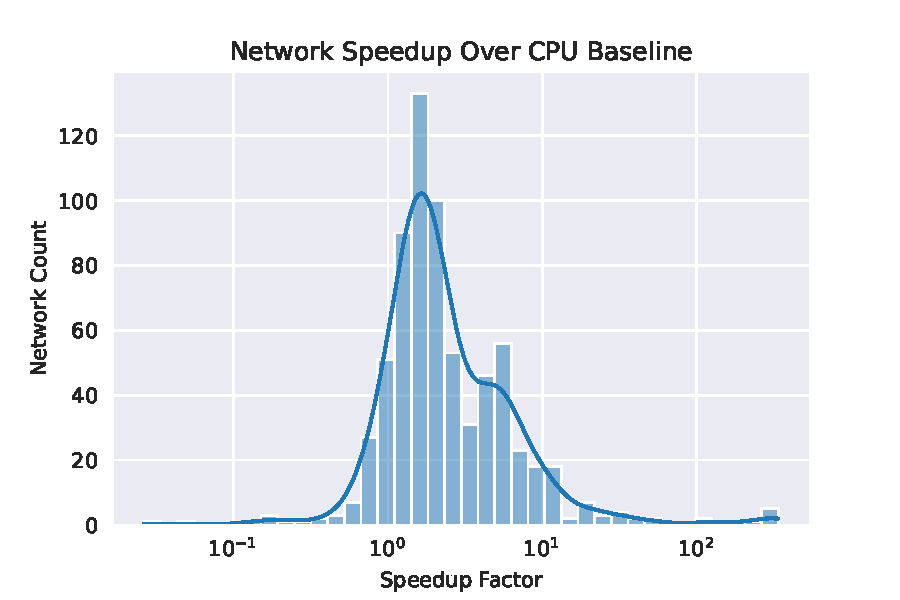
\includegraphics[scale=0.46]{Plots/latency/net_speedup.pdf}
    \hspace{0.1cm} 
    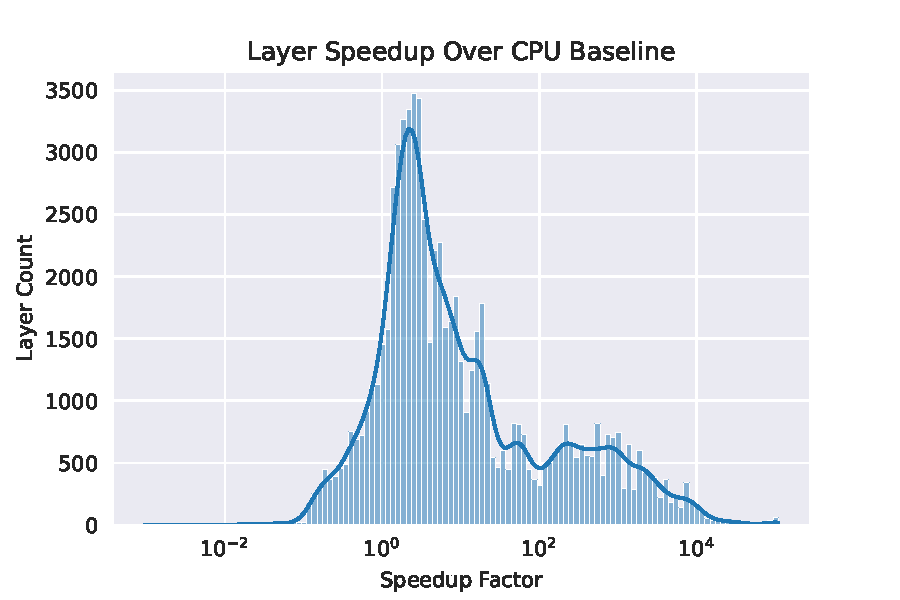
\includegraphics[scale=0.46]{Plots/latency/layer_speedup.pdf}
    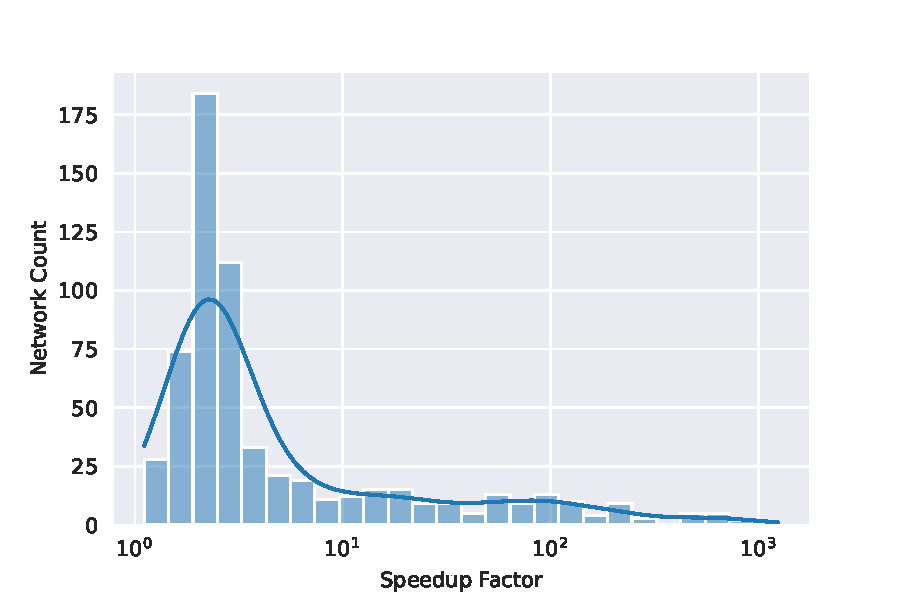
\includegraphics[scale=0.46]{Plots/latency/net_speed_w_offload.pdf}
    \hspace{0.1cm} 
    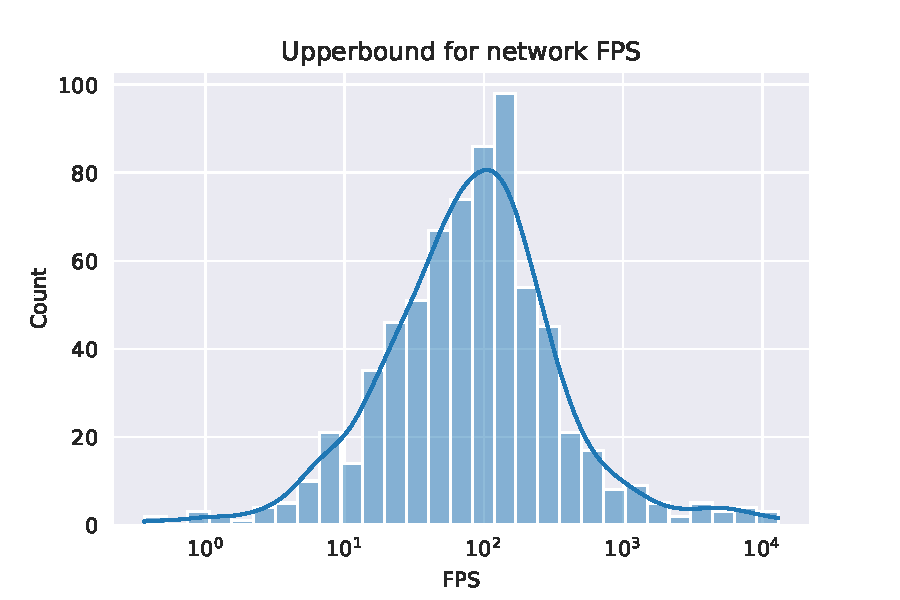
\includegraphics[scale=0.46]{Plots/latency/fps.pdf}
    \caption{a) Histogram of average network speedup over CPU baseline b) Histogram of layer speedup over CPU baseline c) Histogram of average network speedup with offloading of poorly mapped layers with low utilization and low speedup c) Histogram of FPS upper bounds for simulated networks}
    \label{fig:speedup}
\end{figure}

\autoref{fig:speedup}.d  shows the FPS for layers supported by HERO. The median
FPS of supported layers is ~91 FPS with a median speedup of 4.87X over CPU
baseline. Since HERO's support is restricted to convolution and linear
operations these FPS results should serve only as an upper bound estimate for the
actual FPS when running these networks on HERO. An exploration of including
other unsupported layers into HERO is left as part of future work.  

\subsection{DRAM Bandwidth}
\label{chap:hero:results:bw}

\autoref{fig:dram_bw} show the histograms of the load/ store and combined
load store DRAM bandwidth necessary to keep the simulated HERO instance from
stalling. The median required combined DRAM bandwidth is reflected in
\autoref{tab:median_dram_bw}. The maximum combined bandwidth for any network in
the Timm library is 18.3 GiB/s (19.65 GB/s) which is within the ddr4 specification for
PC4-21300 DDR4 SDRAM modules \cite{wiki:List_of_interface_bit_rates} capable of
a 21.3 GB/s transfer rate. 

\begin{figure}[ht]
    \centering
    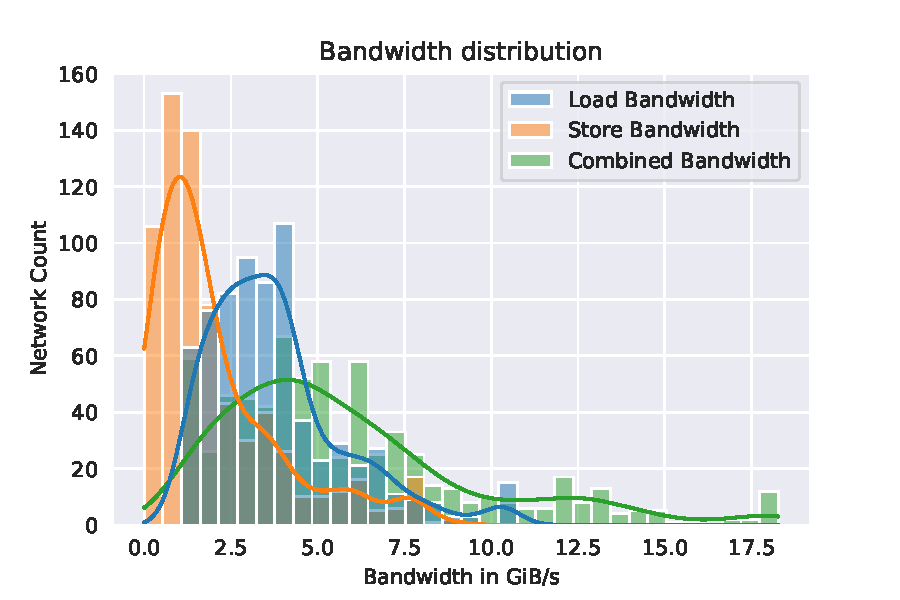
\includegraphics[scale=0.58]{Plots/resources/net_bw.pdf}
    \caption{Hardware Implementation Taxonomy adapted from \cite{maestro}}
    \label{fig:dram_bw}
\end{figure}

\begin{table}[]
    \center
    \begin{tabular}{|l|l|}
    \toprule
    Bandwidth Type. & Bandwidth in GiB/s    \\ 
    \midrule
    Load            & 3.466823  \\ \hline
    Store          & 1.411312  \\ \hline
    Combined          & 4.940233   \\ \hline
\end{tabular}
\caption{Median bandwidth requirements for simulated networks}
\label{tab:median_dram_bw}
\end{table}

\subsection{Energy}
\label{chap:hero:results:energy}

\begin{table}[]
    \center
    \begin{tabular}{|l|l|}
    \toprule
    Operation & Energy Calculation    \\ 
    \midrule
    DRAM Access                 & 160pJ/B  \\ \hline
    On-Chip SRAM Access         & 50+0.022$\sqrt[2]{S}$  \\ \hline
    MAC                         & 767uJ/op  \\ \hline
\end{tabular}
\caption{Energy model from \cite{area_model}}
\label{tab:energy_model}
\end{table}

To estimate energy usage during HERO's operation the energy model from
\cite{area_model} was used. The cost of  on-chip and off-chip communication is
not considered as part of this work. A breakdown of the energy used by different
operations from the energy model in \cite{area_model} is given in
\autoref{tab:hero_config}. Note that while DRAM access and MAC operations are
given as constants multiplied by number of accesses and number of operations,
the access energy for On-Chip sram is a function of the square root of size of
the on-chip SRAM in bits. From \autoref{fig:median_energy_per_network_plot} it's
clear that DRAM energy dominates during an inference of most networks. The
energy consumed by on-chip accesses
of OFmap memory banks is predictably lower than accesses for IFmap banks given
that there's more of them and they are each smaller memories in
comparison to IFmap banks (see \autoref{tab:hero_config}). Reuse chain energy is largely negligible. MAC energy
is non negligible and is similar to weight memory access energy.
\autoref{tab:median_energy_per_network} shows a numerical breakdown of each of
the different operations and the median energy they consumed during inferences
passes of networks in the Timm library. 

\begin{figure}[ht]
    \centering
    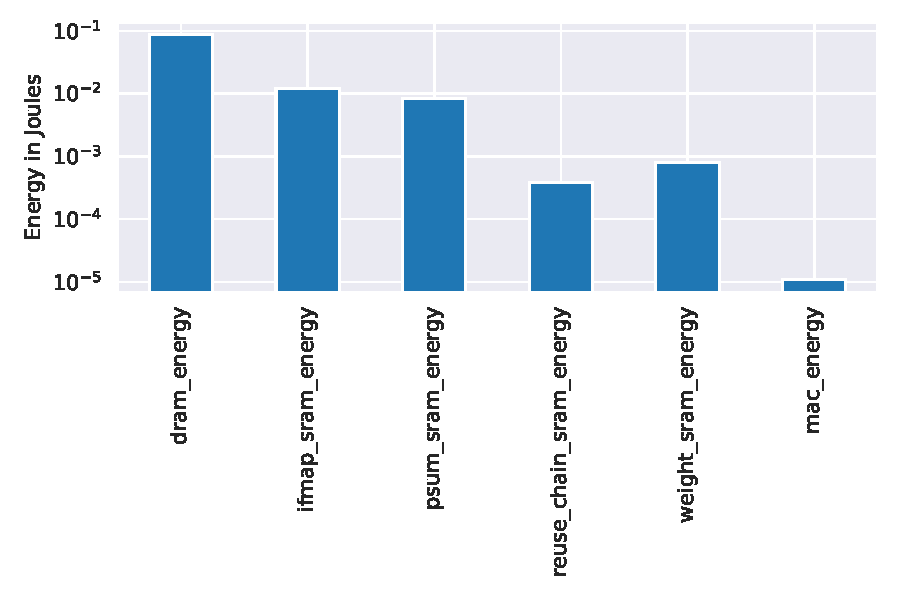
\includegraphics[scale=0.58]{Plots/energy/barplot.pdf}
    \caption{Median network energy breakdown by operation type, note that the vertical axis uses a log scale}
    \label{fig:median_energy_per_network_plot}
\end{figure}

\begin{table}[]
    \center
    \begin{tabular}{|l|l|}
    \toprule
    Operation & Energy Calculation    \\ 
    \midrule
    DRAM access             &  1.725008e-02 J \\
    IFmap SRAM access      &  3.461726e-05 J\\
    OFmap SRAM access        &  1.316624e-05 J\\
    Reuse Chain SRAM access &  7.892650e-07 J\\
    Weight Register access     &  3.130283e-06 J\\
    MAC operation              &  4.778069e-06 J\\
    \bottomrule
\end{tabular}
\caption{Energy model from \cite{area_model}}
\label{tab:median_energy_per_network}
\end{table}

\autoref{fig:inferences_per_j} shows a histogram of the number of inferences/J of
energy consumed. From \autoref{fig:inferences_per_j}.a and
\autoref{fig:inferences_per_j}.b DRAM energy cost is, unsurprisingly, highly influential on
inferences/J. The median inferences/J jumps from 57 Inference/J to 17094
Inferences/J. It's clear that further reducing off-chip data movement by
exploiting more types of concurrency is required. 

\begin{figure}
    \centering
    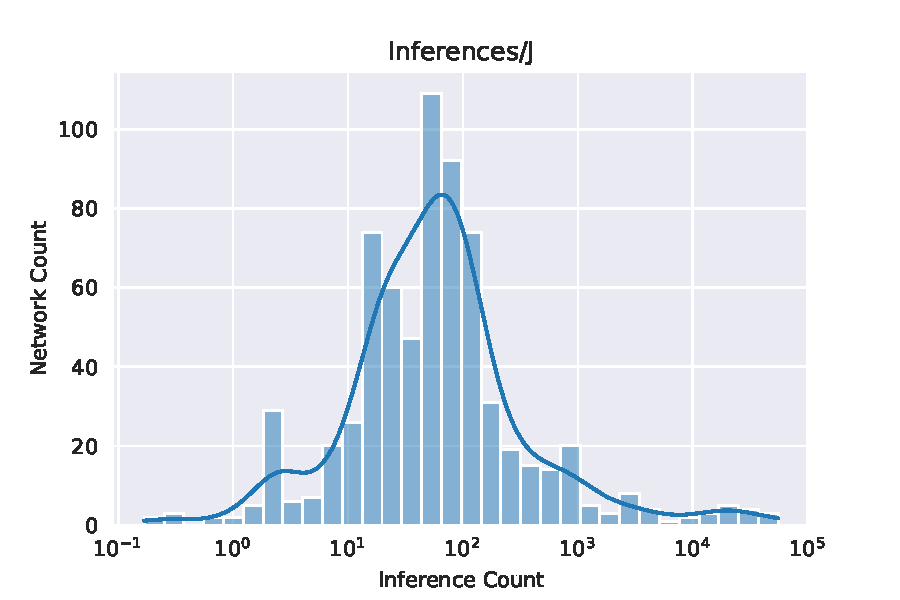
\includegraphics[scale=0.48]{Plots/energy/inferences.pdf}
    \hspace{0.1cm} 
    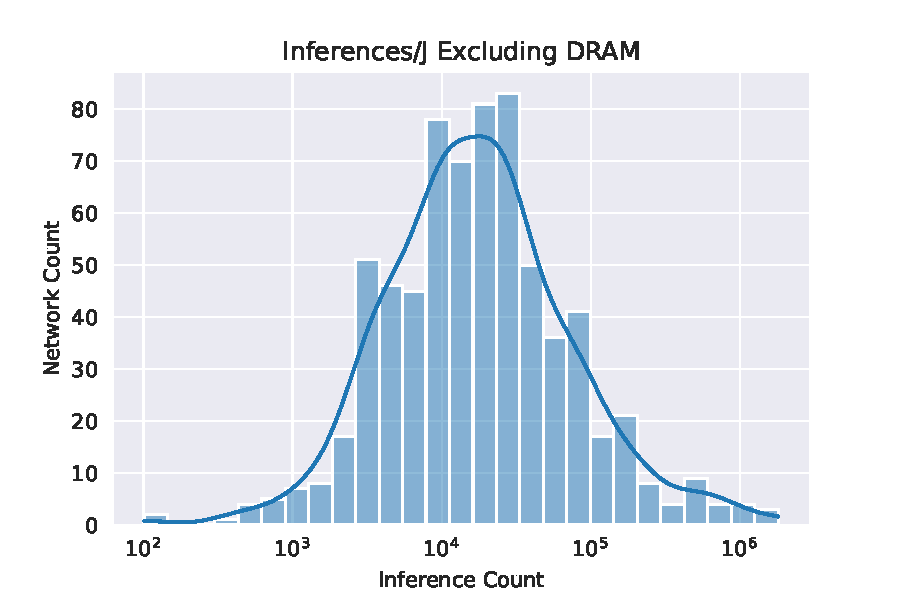
\includegraphics[scale=0.48]{Plots/energy/inferences_wo_dram.pdf}
    \caption{a) Inferences/J when factoring in DRAM access cost b) Inferences/J excluding DRAM access cost}
    \label{fig:inferences_per_j}
\end{figure}

\subsection{Area}
\label{chap:hero:results:area}

To estimate on-chip area for the configurations in
\autoref{tab:hero_config} the area model from \cite{area_model} was used. The area
model from \cite{area_model} is presented in \autoref{tab:area_model_table}.
\autoref{fig:area_breakdown} shows the area model applied to the configuration
in \autoref{fig:area_breakdown} where the vast majority of on-chip area is
consumed by IFmap and OFmap SRAM banks. OFmap memory requires close to double
the area for IFmap memory given the increase in precision required by
accumulation. The total estimated on-chip area required for this configuration
of HERO is 0.34 $mm^2$ using the area model in \autoref{tab:area_model_table}
adapted from \cite{area_model}.

\begin{table}[]
    \center
    \begin{tabular}{|l|l|}
    \toprule
    Unit & On-Chip area    \\ 
    \midrule
    MAC             &  16 $um^2$ \\
    SRAM bit      &  0.013 $um^2/bit$ \\
    \bottomrule
\end{tabular}
\caption{Area model from \cite{area_model} assuming a 14nm technology node}
\label{tab:area_model_table}
\end{table}


\begin{figure}[ht]
    \centering
    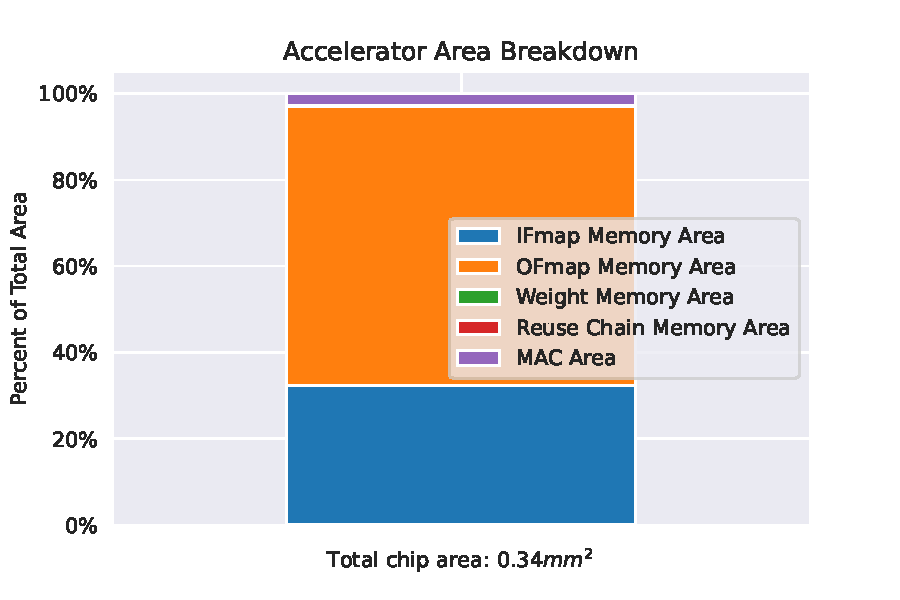
\includegraphics[scale=0.58]{Plots/resources/area.pdf}
    \caption{Area breakdown of HERO in the configuration specified in \autoref{tab:hero_config}}
    \label{fig:area_breakdown}
\end{figure}


\subsection{Per network results}
\label{chap:hero:results:network}

In addition to the library results presented in the previous subsections this
subsections shows the results of running two networks, Resnet50 and Mobilenetv3
on HERO. Resnet50 is a popular image recognition model used as a backbone within
many networks within the Timm library. MobilnetV3 is an image recognition
library developed for low power edge devices. For each network a table is shown
with each layer's configuration. Accompanying the layer breakdown tables are a
series of figures illustrating each network layer's speedup, latency, pe utilization,
energy, bandwidth requirements, and MAC factor increase (in situations were
lowering is required). Note that since each run of HERO is deterministic, layers
with identical configurations are only plotted once. This an important fact to
consider when observing layers with underwhelming performance on HERO. If they
appear infrequently their impact on overall network performance is limited. 

\subsubsection{ResNet50}

From \autoref{tab:resnet50_layer_breakdown}, Resnet50 lacks depthwise layers.
Hence when run on HERO the majority of layers fully utilize the available PEs as
seen in \autoref{fig:resnet50_metrics}. The exception to
this high utilization is conv\_0. Due to it's low channel count and unsupported
kernel types conv\_0 is lowered which substantially increases the MAC count of
the layer. Additionally, because of the large kernel size lowering inflates the
IFmap size necessitating a layer decomposition step that causes PEs to be
underutilized. This causes an overall reduction in layer speedup. The influence
of lowering extends to energy consumption with a few key layers (conv\_6,
conv\_12, conv\_18) consuming the bulk of on-chip energy because of IFmap tensor
size increase. Thankfully these layers occur infrequently in the network and as
a result the majority of layers do not require lowering. The overall estimated
upper bound FPS for resnet50 is 62.7 FPS at 61 Inferences/J and the upper bound of
dram bandwidth required to prevent HERO from stalling falls well below the
PC4-21300 DDR4 SDRAM modules assumed in the energy model discussed in
\autoref{chap:hero:results:energy}. 

\begin{center}
    \begin{table}[]
    \begin{tabular}{lrlrrlllll}
        \toprule
        {} &  Count & IFmap &     Cin &    Cout &       K &  Stride & Padding & Groups &   Bias \\
        Name     &        &             &         &         &         &         &         &        &        \\
        \midrule
        conv\_0   & 1 &  (224, 224) &     3.0 &    64.0 &  (7, 7) &  (2, 2) &  (3, 3) &    1.0 &  False \\
        conv\_1   & 1 &    (56, 56) &    64.0 &    64.0 &  (1, 1) &  (1, 1) &  (0, 0) &    1.0 &  False \\
        conv\_2   & 3 &    (56, 56) &    64.0 &    64.0 &  (3, 3) &  (1, 1) &  (1, 1) &    1.0 &  False \\
        conv\_3   & 4 &    (56, 56) &    64.0 &   256.0 &  (1, 1) &  (1, 1) &  (0, 0) &    1.0 &  False \\
        conv\_4   & 2 &    (56, 56) &   256.0 &    64.0 &  (1, 1) &  (1, 1) &  (0, 0) &    1.0 &  False \\
        conv\_5   & 1 &    (56, 56) &   256.0 &   128.0 &  (1, 1) &  (1, 1) &  (0, 0) &    1.0 &  False \\
        conv\_6   & 1 &    (56, 56) &   128.0 &   128.0 &  (3, 3) &  (2, 2) &  (1, 1) &    1.0 &  False \\
        conv\_7   & 4 &    (28, 28) &   128.0 &   512.0 &  (1, 1) &  (1, 1) &  (0, 0) &    1.0 &  False \\
        conv\_8   & 1 &    (56, 56) &   256.0 &   512.0 &  (1, 1) &  (2, 2) &  (0, 0) &    1.0 &  False \\
        conv\_9   & 3 &    (28, 28) &   512.0 &   128.0 &  (1, 1) &  (1, 1) &  (0, 0) &    1.0 &  False \\
        conv\_10  & 3 &    (28, 28) &   128.0 &   128.0 &  (3, 3) &  (1, 1) &  (1, 1) &    1.0 &  False \\
        conv\_11  & 1 &    (28, 28) &   512.0 &   256.0 &  (1, 1) &  (1, 1) &  (0, 0) &    1.0 &  False \\
        conv\_12  & 1 &    (28, 28) &   256.0 &   256.0 &  (3, 3) &  (2, 2) &  (1, 1) &    1.0 &  False \\
        conv\_13  & 6 &    (14, 14) &   256.0 &  1024.0 &  (1, 1) &  (1, 1) &  (0, 0) &    1.0 &  False \\
        conv\_14  & 1 &    (28, 28) &   512.0 &  1024.0 &  (1, 1) &  (2, 2) &  (0, 0) &    1.0 &  False \\
        conv\_15  & 5 &    (14, 14) &  1024.0 &   256.0 &  (1, 1) &  (1, 1) &  (0, 0) &    1.0 &  False \\
        conv\_16  & 5 &    (14, 14) &   256.0 &   256.0 &  (3, 3) &  (1, 1) &  (1, 1) &    1.0 &  False \\
        conv\_17  & 1 &    (14, 14) &  1024.0 &   512.0 &  (1, 1) &  (1, 1) &  (0, 0) &    1.0 &  False \\
        conv\_18  & 1 &    (14, 14) &   512.0 &   512.0 &  (3, 3) &  (2, 2) &  (1, 1) &    1.0 &  False \\
        conv\_19  & 3 &      (7, 7) &   512.0 &  2048.0 &  (1, 1) &  (1, 1) &  (0, 0) &    1.0 &  False \\
        conv\_20  & 1 &    (14, 14) &  1024.0 &  2048.0 &  (1, 1) &  (2, 2) &  (0, 0) &    1.0 &  False \\
        conv\_21  & 2 &      (7, 7) &  2048.0 &   512.0 &  (1, 1) &  (1, 1) &  (0, 0) &    1.0 &  False \\
        conv\_22  & 2 &      (7, 7) &   512.0 &   512.0 &  (3, 3) &  (1, 1) &  (1, 1) &    1.0 &  False \\
        linear\_0 & 1 &      (1, 1) &  2048.0 &  1000.0 &     N/A &     N/A &     N/A &    N/A &   True \\
        \bottomrule
        \end{tabular}
        \caption{Resent50 layer breakdown}
        \label{tab:resnet50_layer_breakdown}
\end{table}
\end{center}

\begin{figure}[ht]
    \centering
    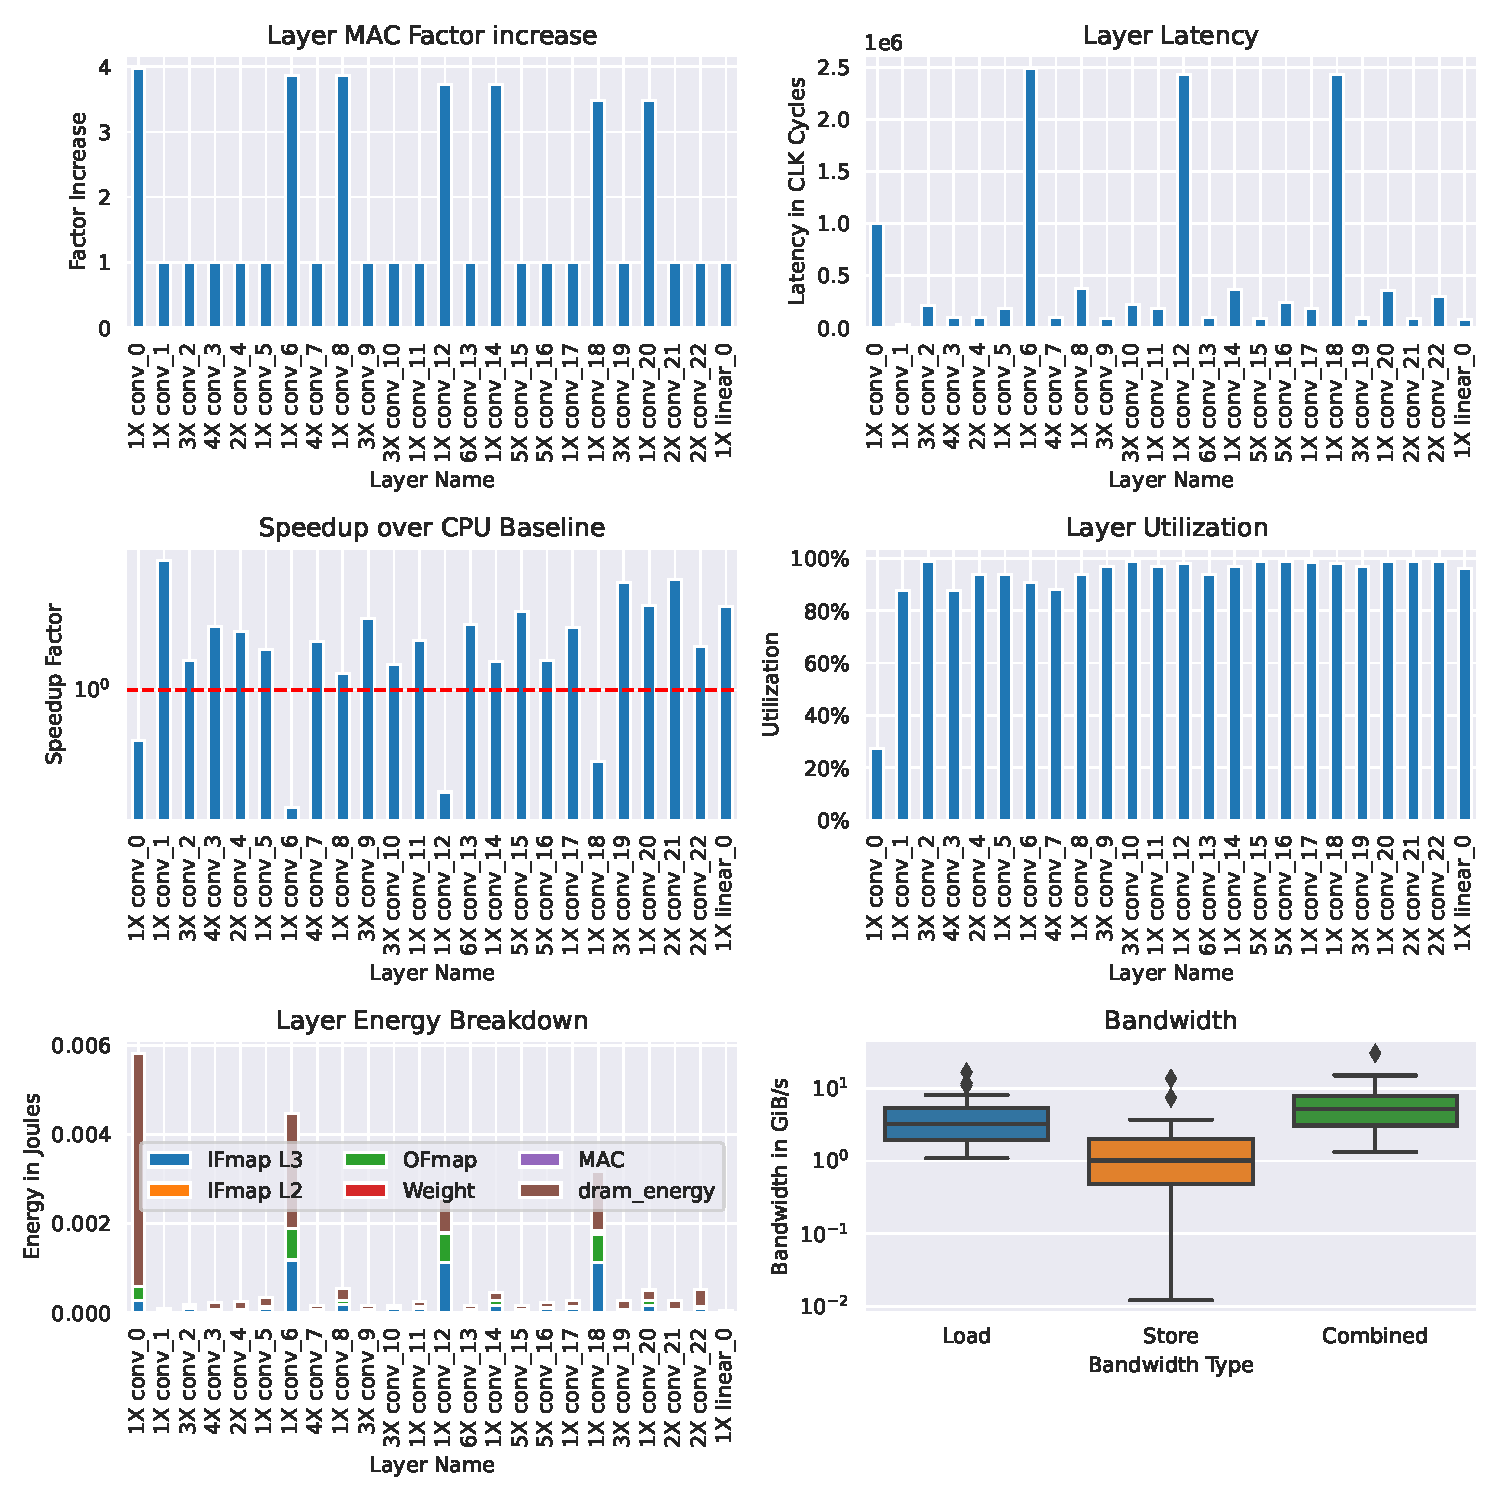
\includegraphics[scale=0.5]{Plots/networks/resnet50.pdf}
    \caption{Resnet50 performance results on HERO with the configuration specified in \autoref{tab:hero_config}}
    \label{fig:resnet50_metrics}
\end{figure}

\subsubsection{MobilenetV3}

From \autoref{tab:mobilenetv3_layer_breakdown}, unlike Resnet50, Mobilenetv3 has
depthwise layers (conv\_1, conv\_6, conv\_12, ...) that map poorly to HERO.
Depthwise layers are supported by running each convolution group sequentially
which greatly diminishes the concurrency advantage of HERO. Depthwise layers
suffer from PE under utilization and substantially reduced speedup over CPU
baseline. Depthwise layers may also require lowering which further reduces their
energy efficiency on HERO. In fact, the layers with the most on-chip energy
consumption are all depthwise layers that have been lowered. Thankfully the
impact of these poorly supported depthwise layers is limited given their
relative infrequency. As a result the overall estimated upper bound FPS for
MobilenetV3 is 928.9 FPS at 328.4 Inferences/J and the upper bound of dram bandwidth
required to prevent HERO from stalling falls well below the PC4-21300 DDR4 SDRAM
modules assumed in the energy model discussed in
\autoref{chap:hero:results:energy}. 


\begin{center}
    \begin{table}[]
    \begin{tabular}{lrlrrlllll}
        \toprule
        {} &  Count &       IFmap &    Cin &    Cout &       K &  Stride & Padding & Groups &   Bias \\
        Name    &        &             &        &         &         &         &         &        &        \\
        \midrule
        conv\_0  &      1 &  (224, 224) &    3.0 &    16.0 &  (3, 3) &  (2, 2) &  (1, 1) &    1.0 &  False \\
        conv\_1  &      1 &  (112, 112) &   16.0 &    16.0 &  (3, 3) &  (2, 2) &  (1, 1) &   16.0 &  False \\
        conv\_2  &      1 &      (1, 1) &   16.0 &     8.0 &  (1, 1) &  (1, 1) &  (0, 0) &    1.0 &   True \\
        conv\_3  &      1 &      (1, 1) &    8.0 &    16.0 &  (1, 1) &  (1, 1) &  (0, 0) &    1.0 &   True \\
        conv\_4  &      1 &    (56, 56) &   16.0 &    16.0 &  (1, 1) &  (1, 1) &  (0, 0) &    1.0 &  False \\
        conv\_5  &      1 &    (56, 56) &   16.0 &    72.0 &  (1, 1) &  (1, 1) &  (0, 0) &    1.0 &  False \\
        conv\_6  &      1 &    (56, 56) &   72.0 &    72.0 &  (3, 3) &  (2, 2) &  (1, 1) &   72.0 &  False \\
        conv\_7  &      1 &    (28, 28) &   72.0 &    24.0 &  (1, 1) &  (1, 1) &  (0, 0) &    1.0 &  False \\
        conv\_8  &      1 &    (28, 28) &   24.0 &    88.0 &  (1, 1) &  (1, 1) &  (0, 0) &    1.0 &  False \\
        conv\_9  &      1 &    (28, 28) &   88.0 &    88.0 &  (3, 3) &  (1, 1) &  (1, 1) &   88.0 &  False \\
        conv\_10 &      1 &    (28, 28) &   88.0 &    24.0 &  (1, 1) &  (1, 1) &  (0, 0) &    1.0 &  False \\
        conv\_11 &      1 &    (28, 28) &   24.0 &    96.0 &  (1, 1) &  (1, 1) &  (0, 0) &    1.0 &  False \\
        conv\_12 &      1 &    (28, 28) &   96.0 &    96.0 &  (5, 5) &  (2, 2) &  (2, 2) &   96.0 &  False \\
        conv\_13 &      2 &      (1, 1) &   96.0 &    24.0 &  (1, 1) &  (1, 1) &  (0, 0) &    1.0 &   True \\
        conv\_14 &      2 &      (1, 1) &   24.0 &    96.0 &  (1, 1) &  (1, 1) &  (0, 0) &    1.0 &   True \\
        conv\_15 &      1 &    (14, 14) &   96.0 &    32.0 &  (1, 1) &  (1, 1) &  (0, 0) &    1.0 &  False \\
        conv\_16 &      2 &    (14, 14) &   32.0 &   192.0 &  (1, 1) &  (1, 1) &  (0, 0) &    1.0 &  False \\
        conv\_17 &      2 &    (14, 14) &  192.0 &   192.0 &  (5, 5) &  (1, 1) &  (2, 2) &  192.0 &  False \\
        conv\_18 &      2 &      (1, 1) &  192.0 &    48.0 &  (1, 1) &  (1, 1) &  (0, 0) &    1.0 &   True \\
        conv\_19 &      2 &      (1, 1) &   48.0 &   192.0 &  (1, 1) &  (1, 1) &  (0, 0) &    1.0 &   True \\
        conv\_20 &      2 &    (14, 14) &  192.0 &    32.0 &  (1, 1) &  (1, 1) &  (0, 0) &    1.0 &  False \\
        conv\_21 &      1 &    (14, 14) &   32.0 &    96.0 &  (1, 1) &  (1, 1) &  (0, 0) &    1.0 &  False \\
        conv\_22 &      1 &    (14, 14) &   96.0 &    96.0 &  (5, 5) &  (1, 1) &  (2, 2) &   96.0 &  False \\
        conv\_23 &      1 &    (14, 14) &   96.0 &    40.0 &  (1, 1) &  (1, 1) &  (0, 0) &    1.0 &  False \\
        conv\_24 &      1 &    (14, 14) &   40.0 &   120.0 &  (1, 1) &  (1, 1) &  (0, 0) &    1.0 &  False \\
        conv\_25 &      1 &    (14, 14) &  120.0 &   120.0 &  (5, 5) &  (1, 1) &  (2, 2) &  120.0 &  False \\
        conv\_26 &      1 &      (1, 1) &  120.0 &    32.0 &  (1, 1) &  (1, 1) &  (0, 0) &    1.0 &   True \\
        conv\_27 &      1 &      (1, 1) &   32.0 &   120.0 &  (1, 1) &  (1, 1) &  (0, 0) &    1.0 &   True \\
        conv\_28 &      1 &    (14, 14) &  120.0 &    40.0 &  (1, 1) &  (1, 1) &  (0, 0) &    1.0 &  False \\
        conv\_29 &      1 &    (14, 14) &   40.0 &   240.0 &  (1, 1) &  (1, 1) &  (0, 0) &    1.0 &  False \\
        conv\_30 &      1 &    (14, 14) &  240.0 &   240.0 &  (5, 5) &  (2, 2) &  (2, 2) &  240.0 &  False \\
        conv\_31 &      1 &      (1, 1) &  240.0 &    64.0 &  (1, 1) &  (1, 1) &  (0, 0) &    1.0 &   True \\
        conv\_32 &      1 &      (1, 1) &   64.0 &   240.0 &  (1, 1) &  (1, 1) &  (0, 0) &    1.0 &   True \\
        conv\_33 &      1 &      (7, 7) &  240.0 &    72.0 &  (1, 1) &  (1, 1) &  (0, 0) &    1.0 &  False \\
        conv\_34 &      3 &      (7, 7) &   72.0 &   432.0 &  (1, 1) &  (1, 1) &  (0, 0) &    1.0 &  False \\
        conv\_35 &      2 &      (7, 7) &  432.0 &   432.0 &  (5, 5) &  (1, 1) &  (2, 2) &  432.0 &  False \\
        conv\_36 &      2 &      (1, 1) &  432.0 &   112.0 &  (1, 1) &  (1, 1) &  (0, 0) &    1.0 &   True \\
        conv\_37 &      2 &      (1, 1) &  112.0 &   432.0 &  (1, 1) &  (1, 1) &  (0, 0) &    1.0 &   True \\
        conv\_38 &      2 &      (7, 7) &  432.0 &    72.0 &  (1, 1) &  (1, 1) &  (0, 0) &    1.0 &  False \\
        conv\_39 &      1 &      (1, 1) &  432.0 &  1024.0 &  (1, 1) &  (1, 1) &  (0, 0) &    1.0 &   True \\
        \bottomrule
        \end{tabular}
        \caption{Mobilenetv3 layer breakdown}
        \label{tab:mobilenetv3_layer_breakdown}
    \end{table}
\end{center}


\begin{figure}[ht]
    \centering
    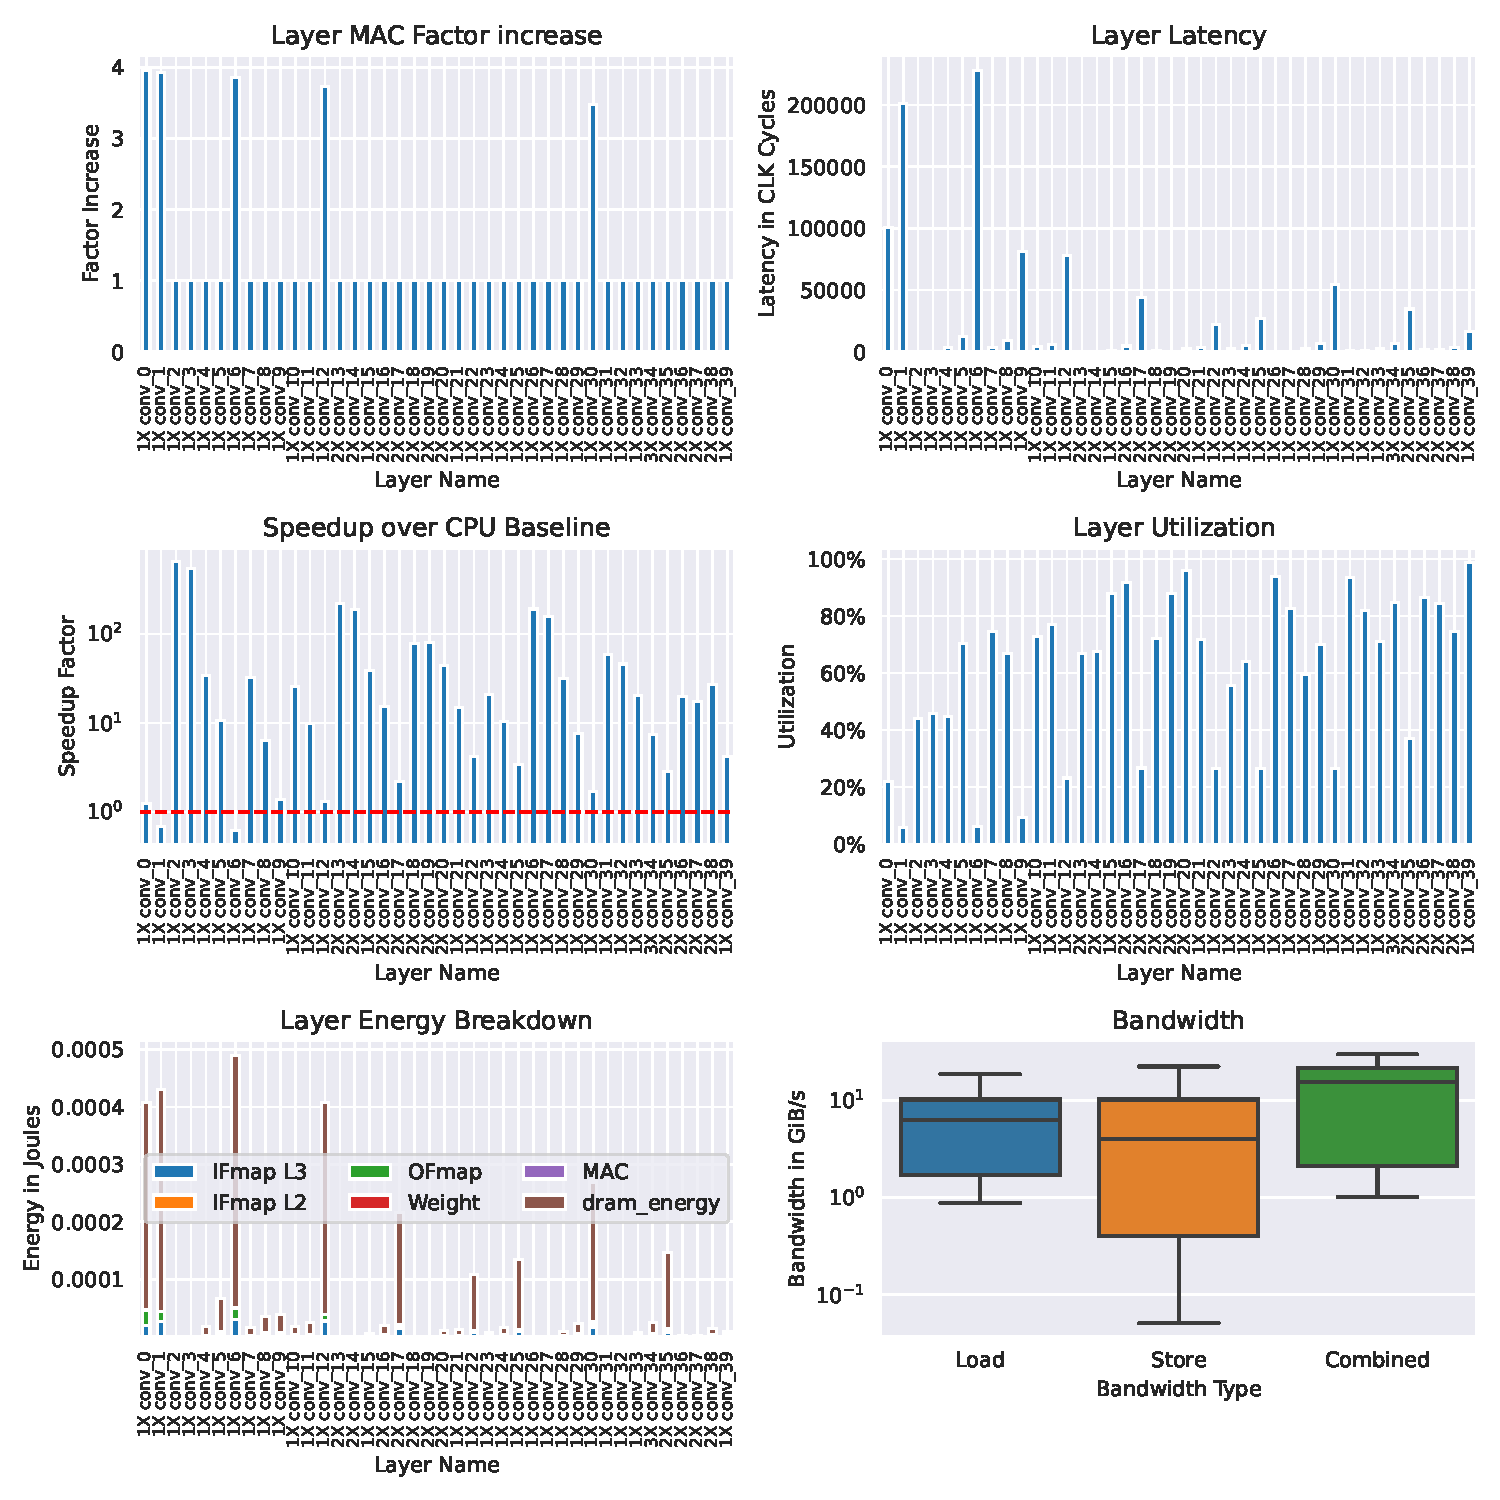
\includegraphics[scale=0.5]{Plots/networks/mobilenetv3_small_075.pdf}
    \caption{Hardware Implementation Taxonomy adapted from \cite{maestro}}
    \label{fig:mobilenetv3_metrics}
\end{figure}



% \subsection{Descriptor program scaling}
% \label{chap:hero:sim_platform:cigar_side}

% median required storage for descriptors per address generator is around 100
% scaling can be improved with more complicated descriptors

% \begin{figure}[ht]
%     \centering
%     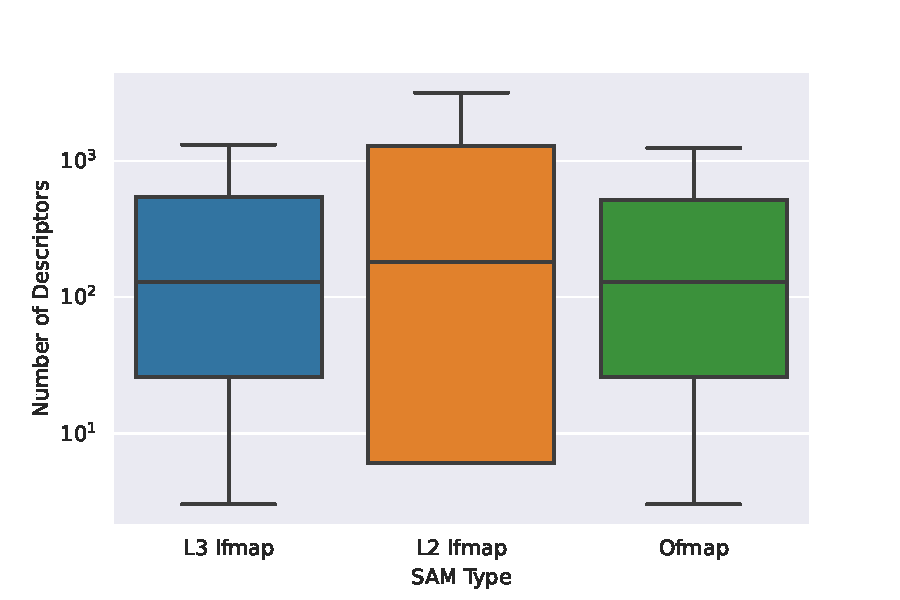
\includegraphics[scale=0.58]{Plots/resources/descriptors.pdf}
%     \caption{Hardware Implementation Taxonomy adapted from \cite{maestro}}
%     \label{fig:hw_taxonomy}
% \end{figure}